\documentclass[11pt]{utalcaDoc}
\usepackage{alltt}
\usepackage{underscore}
\usepackage[utf8]{inputenc}
\usepackage[activeacute,spanish]{babel}
\usepackage{verbatim}
\usepackage[pdftex]{graphicx}
\usepackage{ae}
\usepackage{amsmath}
\usepackage{amsfonts}
\usepackage{pdflscape}
\usepackage{inconsolata}
\usepackage{url}
\usepackage{listings}
% \usepackage{placeins}
\usepackage[section]{placeins}

\title{{\bf Gestión de proyectos tecnológicos}\\ Control ACP}

\author{Erik Regla\\ eregla09@alumnos.utalca.cl}
\date{\today}
\lstset{language=SH, 
		basicstyle=\ttfamily\tiny, 
		showspaces=false, 
		numbers=left, 
		breaklines=true,
		frame=shadowbox
		}

\begin{document}
\maketitle

\section{Justificación del proyecto}

Desarrollo del mercado tecnológico de seguridad informática chileno.

% La oportunidad nace en que ya que Chile ha demostrado ser el campeón de américa y casi de la copa confederaciones, es posible subirse al bandwagon para ahora ser además referentes en ciberseguridad por medio de la creación de un firewall para PYMES de 4ta generación que además de ser un packet filter, logre filtrar los ataques en capa 7.

% El estudio de mercado al cual se hace alusión en el texto indica que las PYMES en general están interesadas en el firewall a desarrollar, al igual que Movistar, VTR y principalmente, CORFO.

\section{Objetivos medibles y criterios de éxito relacionados}


\begin{itemize}
  \item{
    Implementacion del firewall:  
    \begin{itemize}
      \item { El firewall logra frenar ataques en capa 7. }
      \item { El firewall logra cumplir las funciones de packet filter.}
      \item { El core del firewall provisto por snort.com es adaptado exitosamente. }
    \end{itemize}
  }
  % \item{
  %   Aceptación del firewall:
  %   \begin{itemize}
  %     \item { ACTI acepta y aprueba el producto final. }
  %     \item { UChile aprueba y acepta el producto final.}
  %   \end{itemize}
  % }
\end{itemize}

\section{ Restricciones del proyecto }
\begin{itemize}
  \item { Alcance: 
    \begin{itemize}
      \item{ Durante este proyecto no se considera la campaña de marketing. }
      \item { Solo se considera como parte de este proyecto el \textbf{Desarrollo de un prototipo del firewall ``Ni Cagando pasan los Hackers''}.}
    \end{itemize}
  }  
  \item { Tiempo:  
    \begin{itemize}
      \item{ Se dispone de un tiempo de un mes para la instalacion de las oficinas. }
      \item{ Se dispone de un tiempo de tres meses para la adaptación del core. }
      \item{ Se dispone de un tiempo de dos días para el desarrollo del firewall. }
    \end{itemize}
  }  
  \item { Costos: 
    \begin{itemize}
      \item{ El costo del núcleo del firewall tiene un costo de US\$100.000. }
      \item{ El costo de la circuetería requerida es de \$30.000 CLP.}
      \item{ La instalación, configuración y control de calidad sobre la adaptación del firmware tiene un costo de 5UF.}
      \item{ Se dispone de \$7.200.000CLP para contratar programadores para la adaptación del core por 3 meses.}
      \item{ Se dispone de \$2.000.000CLP para contratar pentesters que garantizen la calidad de la modificación del core. }
      \item{ Para el administrativo contratado por 4 meses se dispone de \$2.400.000CLP}
      \item{ Se dispone de \$80.000CLP para sortear los costos de la oficina.}
      \item{ Se dispone de \$260.000CLP para sortear los de arriendo de equipos para el personal.}
      \item{\textbf{ En total se disponen de \$82.100.000CLP para el desarrollo del protoripo.}}
    \end{itemize}
  }  

  \item { Calidad 
    \begin{itemize}
      \item{ El firewall debe poder frenar los ataques en capa 7 con una taza de éxito mayor o igual a la competencia. }
      \item{ El firewall cumple exitosamente las funciones de un packet-filter estándar del mercado con una taza de éxito igual o superior a la competencia.}
    \end{itemize}
  }  
\end{itemize}

\section{Identifique los stakeholders identificando en la matriz Poder/Interés (+o-)}

\begin{figure}[!ht]
  \centering
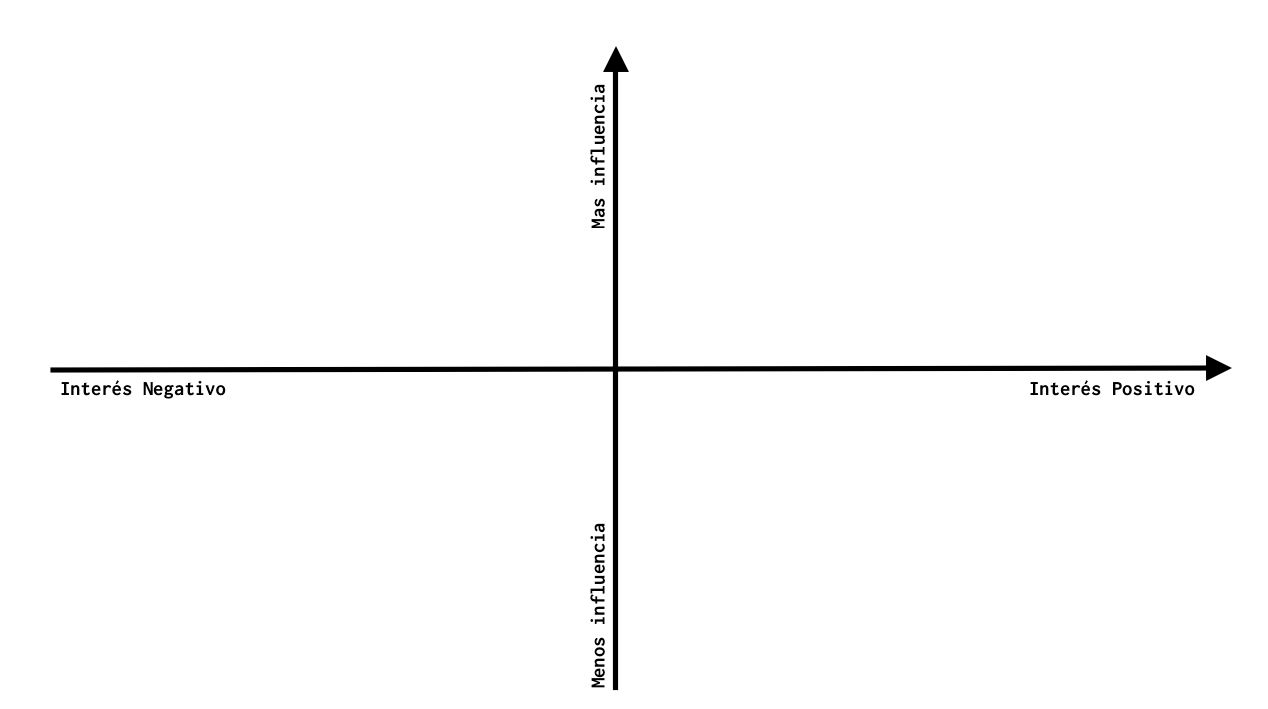
\includegraphics[scale=.3]{tabla.png} 
  \caption{Matriz Poder/Interés}
  \label{FIGURE:MATRIX}
\end{figure}

\section{¿Qué factores externos del proyecto existen?}
\begin{itemize}
  
  \item{Mercado del Dólar.}
  \item{Mercado Chino.}
  \item{Política Empresa Snort.org.}
  \item{Mercado de Servicios Cloud.}
  \item{Mercado de Empresas Pentesting.}
  \item{Legislación Cyberseguridad Chile.}
  \item{Mercado de Programadores en C.}

  % \item{
  %   Cultura organizacional: 
  %   \begin{itemize}
  %     \item{Al ser una organización nueva, existen riesgos debido al poco conocimiento y volatilidad del equipo.}
  %   \end{itemize}
  % }
  % \item{
  %   Legislación Gubernamental: 
  %   \begin{itemize}
  %     \item{ No existe legislación gubernamental al respecto.}
  %   \end{itemize}
  % }
  % \item{
  %   Infraestructura: 
  %   \begin{itemize}
  %     \item{La infraestructura es adquirida.}
  %   \end{itemize}
  % }
  % \item{
  %   Condiciones de mercado: 
  %   \begin{itemize}
  %     \item{Estamos compitiendo con los israelitas, quienes son los líderes en tecnologías de ciberseguridad. Dado que ellos nos tienen mucho más tiempo de ventaja en el mercado, no sabemos si la competencia podría afectar el desarrollo del proyecto al dejar obsoleta la tecnología que estamos desarrollando.}
  %   \end{itemize}
  % }
  % \item{
  %   Clima político: 
  %   \begin{itemize}
  %     \item{ Con la actual crisis política de Corea del Norte, el precio del dolar podría dispararse (o bien derrumbarse) lo cual impacta directamente en los costos del proyecto.}
  %   \end{itemize}
  % }
  % \item{
  %   Tolerancia a riesgos de stakeholders: 
  %   \begin{itemize}
  %     \item{Tanto ACTI como UChile están en contra del proyecto por las repercusiones que podría tener en caso de que el proyecto sea de baja calidad.}
  %   \end{itemize}
  % }
\end{itemize}

\section{Riesgos iniciales de alto nivel del proyecto}{

  \begin{itemize}
    \item{Mala Preparación de Programadores.}
    \item{Aumento del dólar en forma significativa.}
    \item{Falla de Proveedor Pentesting..}
    \item{Falta Dinero para el primer prototipo.}
    \item{No hay elementos(piezas) para armar prototipo.}
    \item{Proveedor no entrega nucleo.}
    % \item{ \textbf{El core del firewall podría no ser compatible con las mejoras requeridas para la completitud del producto:}
    % Para prevenir esto se debe hacer un acuerdo con Snort.org en el cual se indique que el software que ellos ofrecen efectivamente soporta las capacidades que dice de modo de tener un respaldo en caso de que no sea posible. }
    % \item{ \textbf{No logrames adquiri el terreno a corto plazo:}
    % Distender las negociaciones por un periodo mayor de tiempo hasta encontrar un lugar. De otra forma, renegociar con Lusick. }
    % \item{ \textbf{No se logra encontrar desarrolladores capacitados localmente:}
    % Esto obliga a subir el presupuesto para las contrataciones dado que desarrollar este trabajo de manera remota tiene implicancias de seguridad respecto al desarrollo. En especial el diseño de hardware el cual debe ser desarrollado in-situ. }
    % \item{ \textbf{Uno o mas desarrolladores abandonan el proyecto:}
    % Esto obliga a subir el presupuesto para las contrataciones como también a extender el tiempo de desarrollo, dado el impacto que tiene el recambio de personal. Para prevenir los side-effects de esto es necesario un contrato de confidencialidad y exclusividad. }
    % \item{ \textbf{Ocurre un desastre natural en Chile:}
    % Esto detendría el proyecto inmediatamente. Esta opción se considera dado que Chile es un país de desastres. }
  \end{itemize}

}

\end{document}